\section{Uncertainty and Results}
Using the best-performing hyperparameters from the hyperparameter search, % COULDDO: language
the final model is evaluated in more detail.
Specifically,
  the uncertainty of the predictions is analyzed, % Oxford comma
  and the physical plausibility of the predictions is investigated.


\subsection{Bootstrapping}
Bootstrapping \cite{bootstrap} is a method to estimate the uncertainty of a model.
It considers the given data as a random sample from a larger population.
Therefore,
by repeatedly sampling from the data and training a model on each sample,
the model's uncertainty can be determined
as the variance of the results of the different models.
%
For the present work, \num{50} bootstrap samples are used.
Since using a bootstrap sample of the same size as the original (\enquote{bag}) data set
might produce an inconsistent bootstrap estimator \cite{bootstrap_samplesize},
\num{1000000} events are used as the original data set,
while the bootstrap samples contain \num{500000} events as before.


\subsection{Energy Spectrum}
\todo{
  This is (probably) the most important plot. Discuss it in more detail!
}
\autoref{fig:bootstrap:spectrum} shows the unfolded energy spectrum of the optimized model,
as well as the \SI{68}{\percent} confidence intervals,
  ranging from the \SI{16}{\percent} to the \SI{84}{\percent} percentile.
In \autoref{fig:bootstrap:distributions},
the per-bin histograms of the estimations for individual bootstrap runs are shown.
While the probability density in the bins from \SI{E2}{\giga\electronvolt} to \SI{E4}{\giga\electronvolt} is estimated with high precision
  (relative deviation of \SI{6}{\percent} or less apart from the underflow bin),
both the relative deviation and the quantile range are large for the higher energy bins.
It can be speculated that this is due to the fact that the number of events in these bins is small in comparison,
which leads to a large uncertainty in the estimation of the spectrum.
% NOTE: Quadrupling the data set size did not help. :(
%
% TODO: more
% Wasserstein distance
% Accuracy
% MAE
%
The \hyperref[sec:unfolding:metrics:mae]{mean absolute error}… % TODO (this is the only place where it is used so far)

\begin{figure}
  \centering
  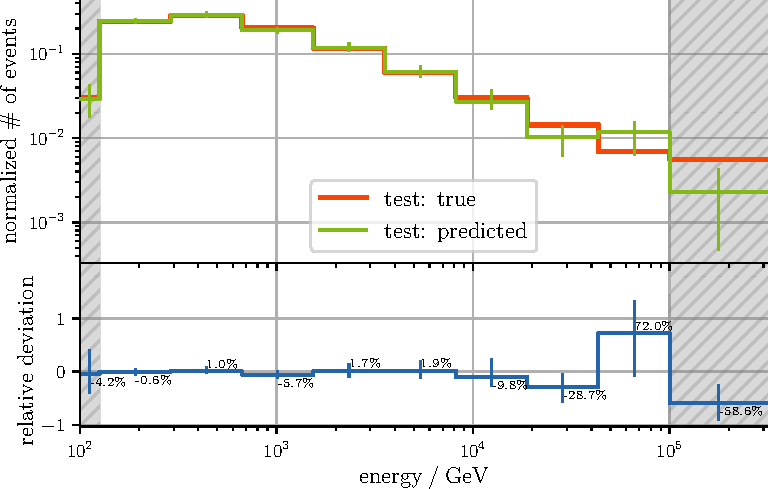
\includegraphics[scale=1]{content/plots/bootstrap:spectrum_full.pdf}
  \caption{
    Energy spectrum and relative deviations of the bootstrap.
    The lines show the median of each bin.
    The error bars indicate the \SI{68}{\percent} confidence intervals,
    ranging from the \SI{16}{\percent} to the \SI{84}{\percent} percentile.
    The greyed out areas mark the under- and overflow bins.
  }
  \label{fig:bootstrap:spectrum}
\end{figure}


\subsection{Individual Events}
Ordinal classification methods promise physically plausible results… % TODO
In contrast to \emph{LogisticAT},
    which \citeauthor{dsea_jan} \cite{dsea_jan} used,
  the unimodality of the probability distribution is not enforced directly.
Instead,
  only the threshold probabilities ($f_k(\mathbf{x}^{[i]})$) are constrained to be monotonically increasing
  by the chain rule of probability
  (see \autoref{sec:corn:method}).
As can be seen in \autoref{fig:bootstrap:single_events},
  slight deviations from unimodality do occur.
Still,
  the indirect constraint on the threshold probabilities
  might be beneficial.

\begin{figure}
  \centering
  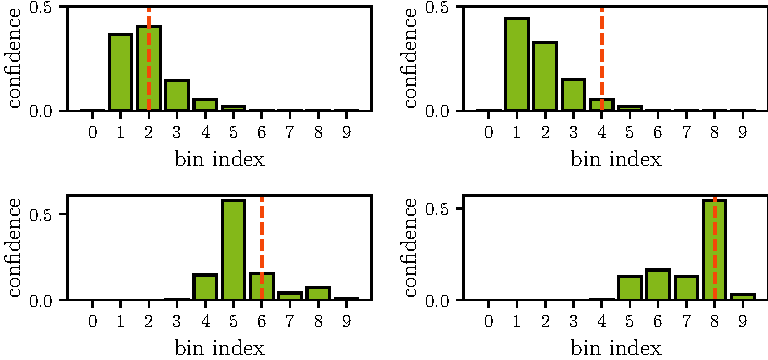
\includegraphics[scale=1]{content/plots/single_events_lessheight.pdf}
  \caption{
    Confidence distributions of selected events.
    The dashed orange line shows the true bin of the event.
    Unimodality is violated with varying severity.
    Two events are misclassified,
      which is indicative of the low accuracy of the model.
  }
  \label{fig:bootstrap:single_events}
\end{figure}

% COULDDO: Compare to a Random Forest?
